\documentclass[12pt,letterpaper]{article}

% --- Paquetes Requeridos ---
\usepackage[utf8]{inputenc}
\usepackage[spanish,es-tabla]{babel}
\usepackage[margin=2.5cm]{geometry}
\usepackage{graphicx}
\usepackage{float}
\usepackage{titlesec}
\usepackage{setspace}
\usepackage{hyperref}
\usepackage{booktabs}
\usepackage{caption}
\usepackage{enumitem}
\usepackage{listings}
\usepackage{xcolor}

% --- Configuración de Párrafo ---
\onehalfspacing
\setlength{\parindent}{0pt}
\setlength{\parskip}{1em}

% --- Rutas de búsqueda de imágenes ---
% Permite compilar tanto desde Documentos/Entregables/ como con todas las
% imágenes en una sola carpeta plana.
\graphicspath{{./}{../Evidencia/}{Evidencia/}{imagenes/}}

% --- Configuración de listings ---
\lstset{
    basicstyle=\ttfamily\footnotesize,
    breaklines=true,
    frame=single,
    captionpos=b,
    showstringspaces=false
}

% --- Inicio del Documento ---
\begin{document}

% --- PORTADA ---
\begin{titlepage}
    \centering

    {\Large \textbf{UNIVERSIDAD SANTO TOMÁS}} \\[1cm]

    {\Large \textbf{Sistema colaborativo de robots móviles para asistencia de orientación en entornos interiores con múltiples pisos}} \\[2cm]

    {\large \textbf{Realizado por:}} \\
    {\large Santiago Hernández Ávila} \\
    {\large Jonny Alejandro Mejía León} \\[1cm]

    \begin{figure}[H]
        \centering
        \includegraphics[width=0.6\textwidth]{Logos Uni.png}
        \label{Logo Universidad Santo Tomas y facultad de ingenieria electronica}
    \end{figure}

    \vfill

    {\large \textbf{Informe de Avance --- Semana 22}} \\
    {\large Fase 5: Integración del sistema y realización de pruebas --- Cierre de la interfaz humano--robot sobre un teléfono real y caracterización de la cadena de mapeo} \\[1.5cm]

    \textbf{Dirigido por:} \\
    Ing. Armando Mateus Rojas, Msc. \\
    Ing. Nestor Ivan Ospina, Msc. \\
    Ing. Oscar Mauricio Gélvez Lizarazo, Msc. \\[1.0cm]

    \vfill

    {\large GED (Grupo de Estudio y Desarrollo en Robótica)} \\
    {\large Facultad de Ingeniería Electrónica} \\
    {\large División de Ingenierías} \\
    {\large Bogotá, septiembre de 2026}
\end{titlepage}

% --- CONTENIDO ---

\section{Introducción}

El presente informe documenta el avance correspondiente a la \textbf{Semana 22} del cronograma de actividades (7 al 13 de septiembre de 2026), dentro de la \textbf{Fase 5 (Integración del sistema y realización de pruebas)}.

Es la semana en que el sistema queda \textbf{completo de extremo a extremo}: el 10 de septiembre una persona seleccionó origen y destino desde un teléfono móvil real y el sistema completó el guiado con relevo entre niveles sin intervención manual. Ese es, palabra por palabra, el criterio de cierre que el cronograma fija para esta semana, y se cumplió con un registro validado en lugar de con una declaración. Se expone en la Sección \ref{sec:hri}.

La semana produjo además \textbf{tres resultados de método} que el informe considera tan relevantes como el criterio cumplido, y que comparten una misma forma: en los tres casos se midió el mecanismo antes de decidir.

El primero es el frente de hardware. Su medición de aceptación (G2) se intentó por segunda semana consecutiva y \textbf{volvió a quedarse sin veredicto}: cuatro grabaciones produjeron cuatro mapas rechazados. Pero la salida no terminó ahí: la hipótesis que se traía al campo ---``el vehículo se movió demasiado rápido''--- quedó \textbf{refutada por la propia medida}, y el mecanismo real se caracterizó el mismo día. De paso salió el \textbf{primer mapa que este proyecto acepta con SLAM}. Se expone en la Sección \ref{sec:mapeo}.

El segundo es el cierre del riesgo R12. La campaña experimental de la semana anterior había dejado una misión anómala con 85 cúspides frente a una mediana de 7, atribuida provisionalmente al comprobador de meta. \textbf{No era eso}, y la causa real está ahora localizada en una línea del controlador de Nav2. Se expone en la Sección \ref{sec:r12}.

El tercero es el más incómodo de escribir y por eso se escribe: un barrido sistemático del protocolo experimental encontró que \textbf{la variable de respuesta principal del objetivo 4 no puede dar ``no''}. Su criterio binario es verdadero por construcción, de modo que sus 30 verificaciones en verde no son evidencia de nada. No cambia ningún veredicto de la campaña, pero sí cambia cómo debe redactarse el capítulo de resultados. Se expone en la Sección \ref{sec:barrido}.

\section{Objetivos de la Semana}

El cronograma fija para esta semana el siguiente criterio de cierre:

\begin{quote}
\textit{Desde un teléfono se selecciona origen y destino, y el sistema completa el guiado con relevo en simulación sin intervención manual.}
\end{quote}

Las actividades planificadas eran cuatro: la interfaz web responsiva sobre \texttt{rosbridge\_suite} (objetivo 3), la integración de los cuatro módulos de extremo a extremo en simulación, el despliegue sobre los vehículos físicos según el resultado del punto de decisión, y la emisión del informe de la Semana 21.

\textbf{El criterio de cierre se cumplió el 10 de septiembre}, con evidencia registrada y no con declaración. El despliegue sobre los vehículos físicos \textbf{no se ejecutó}, porque depende de un punto de decisión que sigue abierto por razones que la Sección \ref{sec:mapeo} documenta.

\section{La interfaz humano--robot queda cerrada sobre un teléfono real}
\label{sec:hri}

\subsection{Qué separaba ``verificado'' de ``cerrado''}

La interfaz llevaba desde el 2 de septiembre verificada contra un coordinador real, pero siempre desde el navegador del computador portátil. Ese escenario \textbf{no} es el que el requisito RF-20 pide: el requisito exige un dispositivo móvil físico, y la diferencia no es cosmética. Un navegador de escritorio y uno de teléfono difieren en el ancho de la ventana, en el modelo de eventos táctiles y ---lo que resultó decisivo--- en que el teléfono está en otra máquina de la red, de modo que tiene que atravesar el cortafuegos del anfitrión.

\subsection{El procedimiento de red, que no estaba escrito en ninguna parte}

Para que la página cargara en el móvil hubo que abrir los puertos 8000 (servidor de la página) y 9090 (puente de ROS) en \texttt{ufw}, y se abrieron \textbf{acotados a la subred}, no al aire. La razón se deja escrita porque es una decisión de seguridad y no una preferencia: \texttt{rosbridge} \textbf{no tiene autenticación}, de modo que publicarlo sin restricción de origen equivale a entregar el mando de los dos robots a cualquiera que pase por el pasillo con un teléfono.

El procedimiento completo no constaba en ningún documento del repositorio ---se había ejecutado de memoria cada vez--- y quedó incorporado como \S 4.1 de \texttt{RUNBOOK\_CAMPANA.md}.

\subsection{La distinción entre ``carga'' y ``sirve''}

La página cargó en el móvil sobre el SSID \texttt{DEEPRACER} y el indicador de conexión se puso verde, lo que significa \textbf{WebSocket establecido} contra \texttt{rosbridge} y no solamente HTML servido. Aun así, eso todavía no cierra RF-20: una página que carga no es una página que opera.

Esa misma tarde se operó una misión completa desde el teléfono: \texttt{piso1\_etm2} $\rightarrow$ \texttt{piso2\_aula\_302}, con los dos robots vivos y relevo entre niveles. \textbf{La evidencia no es la pantalla sino el registro validado} \texttt{S22\_RF20\_telefono\_C\_02.json}, que reporta \texttt{exito: true}, \texttt{c3\_relevo: true}, continuidad sin huecos y un factor de tiempo real de 0,9949.

Con esto \textbf{RF-17 a RF-20 quedan los cuatro verificados} y cae el criterio de cierre de la semana.

\subsection{RF-28: el segundo tramo arrancaba con el usuario todavía en el otro piso}
\label{sec:rf28}

Este requisito no existía al abrir la semana. Sale de la primera de cinco situaciones de usuario que la dirección planteó para la interfaz, y \textbf{el defecto era de diseño, no de código}.

La secuencia de una misión entre niveles termina la etapa de transferencia cuando el robot del piso de destino llega a su escalera. Pero el robot no puede saber si \textbf{la persona} ya subió. Sin una pausa explícita, la misión podía declararse completada con el usuario todavía en el piso equivocado ---un fallo que la instrumentación habría registrado como éxito, porque el robot sí llegó.

La corrección añade la etapa \texttt{ESPERANDO\_CONFIRMACION = 7} a la máquina de estados de la misión, con una regla que merece enunciarse porque protege de un fallo sutil: \textbf{cualquier confirmación anterior deja de valer al empezar una misión nueva}. Sin esa regla, una pulsación tardía de la misión anterior arrancaría el segundo tramo de la siguiente sin preguntar.

\textbf{Lo probable sin simulador se probó sin simulador}: política de plazos, enganche de la confirmación, y una regresión que verifica que la etapa 7 \textbf{no altera ni la continuidad ni el hueco de relevo}. Esta última es la comprobación que impide que un requisito nuevo estropee una métrica ya medida, y por eso se escribió antes que el código de la interfaz.

\textbf{El hallazgo del día fue de otra clase.} El botón de confirmar parecía no funcionar, y el fallo no era suyo: \texttt{rosbridge} atiende en un \textbf{hilo único}, de modo que la publicación quedaba encolada detrás de la llamada bloqueante que se estaba sirviendo. Es la misma familia de defecto que los dominios DDS del 30 de agosto ---el síntoma es silencio y el culpable aparente es siempre el último componente que se tocó. Las tres corridas de evidencia están en \texttt{S22\_RF28\_confirmacion.md}, con las etapas extraídas del registro en bruto mediante \texttt{inspeccionar\_etapas.py} y \textbf{no leídas de la pantalla}.

\subsection{El defecto que queda abierto, y por qué el objetivo 3 no llega al 100 \%}

La cancelación de una misión en curso \textbf{no funciona}: el nodo coordinador no declara callback de cancelación y la interfaz se queda indefinidamente mostrando ``Enviando la cancelación\ldots''. No lo cubre ningún requisito ---nadie escribió un RF de cancelación--- pero \textbf{se ve en pantalla}, que es el criterio que importa en una interfaz de usuario.

Por eso el objetivo 3 sube del 35 \% al \textbf{90 \%} y no al 100 \%. La decisión de si se corrige depende del calendario: la congelación de código es el 20 de septiembre, y compite con otros dos frentes.

\section{Frente de hardware: el mapa que no salió, y el primero que sí}
\label{sec:mapeo}

\subsection{Cuatro grabaciones, cuatro mapas rechazados}

El Bloque 3 de la medición G2 ---la pasada que produce el mapa contra el cual se miden las dos cifras de aceptación--- se ejecutó \textbf{cuatro veces} el 8 de septiembre y \textbf{ninguna produjo un mapa aceptable}. Los bloques posteriores no se ejecutaron, por aplicación de la regla preinscrita en el \S 7 de la hoja de campo: \textbf{sin mapa aceptado no hay contra qué localizarse}.

Conviene subrayar que ninguna de las cuatro grabaciones está vacía: las cuatro superan el comprobador de movimiento, y las cuatro se conservan. El problema no fue de captura.

\subsection{La hipótesis que se traía, refutada por la propia medida}

Se llegó al campo con una explicación de la semana anterior: el vehículo se movió demasiado rápido. Se midió en lugar de suponerse. Alineando cada barrido del sensor con el siguiente ---buscando el desplazamiento angular que minimiza la diferencia mediana de rangos--- se obtienen dos cifras por grabación: cuánto gira el sensor entre barridos, y cuánto residuo queda \textbf{después} de alinear.

\begin{table}[H]
    \centering
    \small
    \caption{Las cuatro pasadas del Bloque 3 sobre la recta de ensayo de 20,00 m.}
    \label{tab:pasadas}
    \begin{tabular}{@{}lcccl@{}}
        \toprule
        \textbf{Bag} & \textbf{Modo} & \textbf{Giro mediano} & \textbf{Residuo} & \textbf{Mapa obtenido} \\ \midrule
        \texttt{2046} & empujado  & 0,0 $^\circ$/s  & 0,037 m & 1166 $\times$ 267 m \\ \addlinespace
        \texttt{0012} & empujado  & 0,0 $^\circ$/s  & 0,035 m & 47,5 $\times$ 29,1 m \\ \addlinespace
        \texttt{2029} & conducido & 13,9 $^\circ$/s & 0,085 m & 95 $\times$ 36 m \\ \addlinespace
        \texttt{2009} & conducido & 20,8 $^\circ$/s & 0,099 m & 62 $\times$ 52 m \\ \bottomrule
    \end{tabular}
\end{table}

Conducir \textbf{sí} degrada el dato: el residuo entre barridos se triplica frente a empujar. Pero \textbf{el orden se rompe}: la pasada más suave de las cuatro produjo el peor mapa, por un factor de veinte. Si el movimiento fuese la causa, \texttt{2046} debería haber sido el mejor.

Esa refutación es también la que justifica \textbf{cerrar la salida en lugar de repetirla}. Con el movimiento cubriendo todo el rango de suave a brusco y el fallo presente en los cuatro casos, más pasadas no aportan información nueva.

\begin{figure}[H]
    \centering
    
\includegraphics[width=0.47\textwidth]{S22_mapa_2046_fallido.png}
    \hfill
    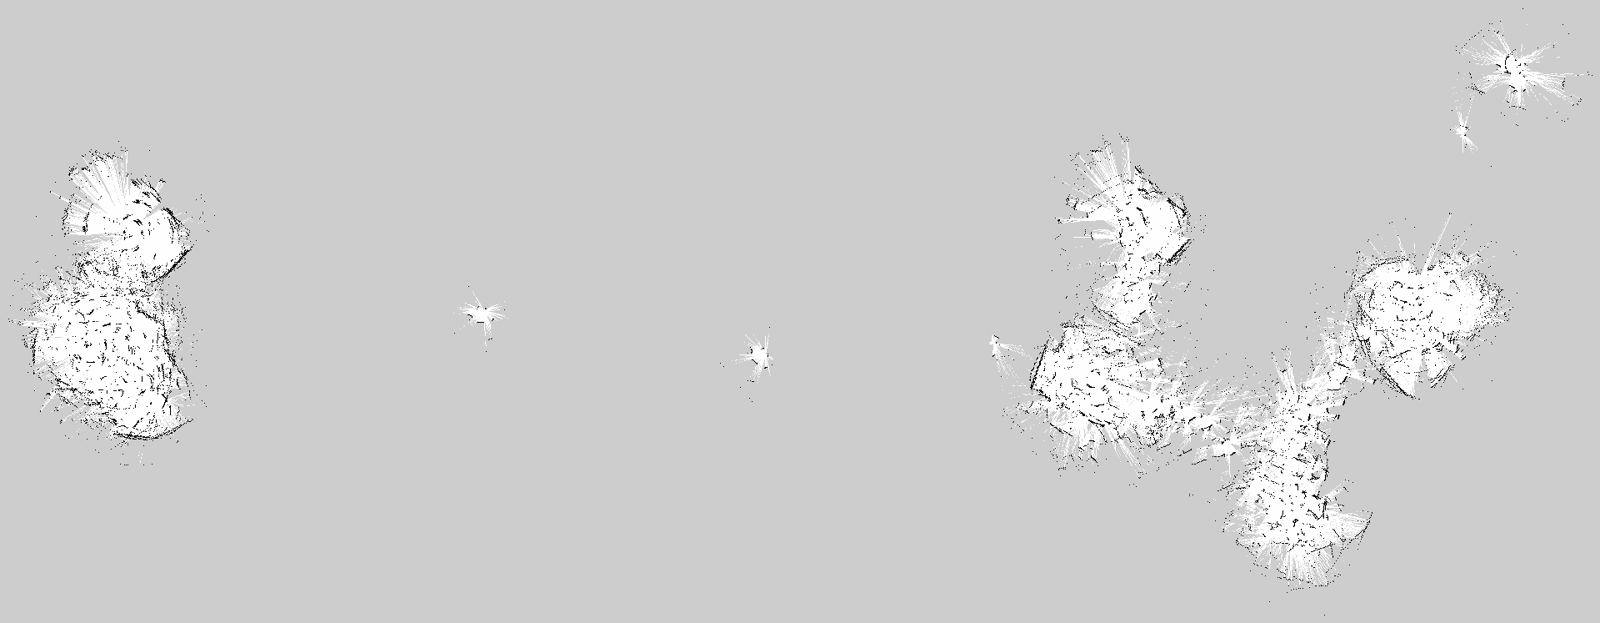
\includegraphics[width=0.47\textwidth]{S22_mapa_2029_fallido.png}
    \caption{Izquierda: la pasada más suave (\texttt{2046}), que produce un mapa de 1166 m de extensión. Derecha: una pasada conducida (\texttt{2029}). El movimiento brusco no explica la diferencia.}
    \label{fig:mapas_fallidos}
\end{figure}

\subsection{El mecanismo, medido: la información de avance no está en el dato}

La pregunta que faltaba no era ``¿el mapa está mal?'' sino ``¿por qué?''. Se contesta descomponiendo el desplazamiento estimado \textbf{en el marco del robot}, ventana a ventana de un segundo, contra la verdad de terreno del mismo registro.

\begin{quote}
Longitudinal \textbf{0,388} \quad$\cdot$\quad Lateral \textbf{1,143} \quad$\cdot$\quad Rotación \textbf{1,055}
\end{quote}

Esa descomposición es la que decide, y por una razón precisa: \textbf{un error de escala afecta a todo por igual, y una inobservabilidad no}. Lo lateral y el giro se estiman bien; \textbf{solo se pierde el avance}. Con eso caen simultáneamente todas las causas que afectarían al barrido entero ---el reloj, las transformadas, los fallos de deserialización.

Y la pérdida \textbf{es un interruptor, no una deriva}. Por bloques de 30 s la razón salta entre 0,997 / 0,999 / 0,817 y 0,068 / 0,085 / 0,111. Agrupando por lo que el sensor tiene delante: \textbf{0,998 con estructura a menos de 6 m, y 0,255 entre 6 y 9 m}. En las ventanas ciegas el alcance frontal está \textbf{clavado en 7,40 m mientras el robot avanza 1,00 m}, y no es saturación ---el sensor simulado alcanza 10,0 m. Es la pared lateral vista por el borde del sector, a distancia invariante.

El mecanismo queda entonces sin hueco: la odometría láser estima el movimiento \textbf{solo} del cambio entre barridos consecutivos, y en un pasillo recto y uniforme cada rango queda determinado por la posición lateral y el rumbo, \textbf{no por la longitudinal}. El robot avanza, el barrido siguiente es idéntico al anterior, y el estimador devuelve casi cero ---y \textbf{acierta}, porque desde el punto de vista del sensor no ha pasado nada.

No es un defecto del algoritmo ni un parámetro mal puesto. \textbf{La información no está en el dato.} Es la inobservabilidad longitudinal que el proyecto ya tenía caracterizada sobre la localización, medida ahora directamente sobre la cadena de mapeo.

\subsection{El ensayo controlado, y el primer mapa aceptado del proyecto}

Antes de esta semana, \textbf{nadie había aceptado nunca un mapa en este proyecto} ---ni en simulación. Mientras eso fuera cierto, era imposible distinguir un fallo del pasillo de un fallo de la cadena. Ese experimento se montó la misma tarde, con criterio y predicción escritos \textbf{antes} de correr, como exige el \S 6.3 del protocolo.

El banco: una caja \textbf{cerrada} de 7,70 $\times$ 2,70 m, donde las dos paredes de los extremos entran siempre en el alcance del sensor. Recta pura de ida y vuelta, cuatro travesías, 22,4 m a 0,33 m/s, \textbf{sin un solo giro} ---el mismo movimiento y la misma velocidad que fallaron en el pasillo largo, de modo que \textbf{la única variable es la geometría del entorno}.

\begin{quote}
La razón de desplazamiento sube de \textbf{0,209 a 1,010}, y el mapa da \textbf{98,1 \% en X, 95,0 \% en Y y 0 de 755 obstáculos inventados: ACEPTADO}.
\end{quote}

\begin{figure}[H]
    \centering
    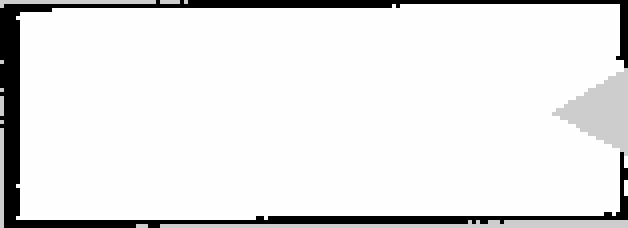
\includegraphics[width=0.6\textwidth]{S22_mapa_caja_SIMULACION_aceptado.png}
    \caption{Primer mapa aceptado por la cadena SLAM del proyecto, sobre la caja cerrada en simulación. La verdad de terreno es exacta porque procede del propio simulador.}
    \label{fig:mapa_aceptado}
\end{figure}

\textbf{La cadena funciona.} Y la condición para que funcione pasa a ser \textbf{medible antes de salir}: estructura no uniforme dentro del alcance del sensor durante todo el recorrido.

\subsection{Dos defectos que salieron de que el mapa se rechazara al primer intento}

Ninguno de los dos era de SLAM, y los dos habrían envenenado cualquier mapa futuro:

\begin{enumerate}[leftmargin=*]
    \item \textbf{El umbral de celda libre.} La herramienta de guardado escribe \texttt{free\_thresh: 0.25} y el valor 205 para ``desconocido''. Pero 205 corresponde a 0,196 de ocupación, \textbf{por debajo de 0,25}: el servidor de mapas lee como \textbf{libre} cada celda que el mapa declara desconocida, y el planificador traza rutas por donde nadie ha mirado. Los mapas vigentes del repositorio traen 0,1; los de esta cadena, no.

    \item \textbf{El origen del mapa no está en el origen del mundo.} SLAM sitúa el marco del mapa \textbf{donde arrancó el vehículo}. El robot nació en $x = -3{,}0$, el mapa salió corrido 3 m, y el verificador reportó \textbf{el 47 \% de los obstáculos como inventados}. Restado el corrimiento: \textbf{0,0 \%}. Es una trampa seria ---el mapa es correcto y el informe dice que está lleno de paredes falsas--- y ahora el guion avisa.
\end{enumerate}

\subsection{Un hallazgo de fondo sobre el sensor, y qué queda del punto de decisión}

La jornada dejó además dos cosas medidas sobre el hardware que no estaban documentadas. La primera: \textbf{el sector ciego del LiDAR mide $\sim$90$^\circ$, no los 60$^\circ$ que declara el modelo}, y apunta al eje del pasillo. La segunda, que es la que hay que resolver antes de volver al campo: \textbf{hay 180$^\circ$ de discrepancia entre el modelo y el montaje real}. El modelo declara un hueco hacia el frente del vehículo; en las grabaciones el sector ciego aparece alrededor del cero del marco del sensor. No es cosmético ---si el sensor va montado al revés que el modelo, la odometría láser entrega el avance con el signo cambiado, que es mecanismo suficiente para producir un mapa de 1166 m.

\textbf{El punto de decisión GO/NO-GO sigue abierto, por segunda semana consecutiva}, y esta vez no por un olvido de calendario sino porque el pasillo no da mapa. Lo siguiente \textbf{no requiere conducir el vehículo}: traer al computador las grabaciones del 7 de septiembre y aplicarles esta misma medida, y tomar con flexómetro el largo real del pasillo y dónde están sus rupturas ---puertas, columnas, cruces, cambios de ancho. Es trabajo de libreta, no de robot.

\subsection{Una cifra correcta con la etiqueta equivocada}

Se deja escrita una lección de método que se cobró esta semana. Se afirmó que ``el pasillo mide 20,08 m y el LiDAR alcanza 12,0 m, luego está mejor condicionado que el simulado de 46,9 m''. \textbf{Es falso}: los 20,00 m son el largo de la \textbf{recta de ensayo} marcada con cinta, que es el mensurando de la medición, \textbf{no la geometría del edificio}. El pasillo es bastante más largo y nadie lo ha medido.

La corrección además apunta al lado desfavorable: una recta de 20 m contenida dentro de un pasillo uniforme mucho más largo es \textbf{exactamente} la geometría que falla. \textbf{Una cifra correcta con la etiqueta equivocada produce una conclusión falsa igual de bien que un dato malo}, y esta llegó a escribirse en tres sitios antes de detectarse.

\section{Cierre del riesgo R12: las 85 cúspides}
\label{sec:r12}

La campaña del objetivo 4 dejó 29 misiones con una mediana de 7 cúspides ---maniobras de inversión de marcha--- y \textbf{una con 85}. La atribución provisional era el comprobador de meta. \textbf{No era eso.}

La causa está localizada: la opción que permite marcha atrás activa una comprobación de cúspide en el controlador, que reduce la distancia de anticipación de 0,600 m a \textbf{0,0165 m}. Con esa anticipación, el cuadrado de la distancia al punto objetivo vale $2{,}71 \times 10^{-4}$, que cae \textbf{por debajo} de la guarda de $10^{-3}$ ---equivalente a 3,16 cm. La curvatura queda entonces exactamente en cero: \textbf{la dirección deja de actuar}, mientras el sentido de marcha sigue invirtiéndose según el signo de una coordenada de 1,6 cm.

Lo que cierra el diagnóstico es que \textbf{el caso de control está en la misma grabación}: el otro robot atravesó una cúspide a 91,4 mm ---fuera de la guarda--- y la resolvió en 3,5 s. Mismo código, misma misión, mismo instante; la única diferencia es de qué lado de los 3,16 cm cayó el punto objetivo.

R12 queda \textbf{cerrado}. La documentación completa está en \texttt{S22\_R12\_85\_cuspides.md}.

\section{Barrido del protocolo: un criterio que no puede fallar}
\label{sec:barrido}

\subsection{Por qué se hizo el barrido}

El proyecto ya había tropezado dos veces con la misma clase de defecto. Una métrica que valía cero por construcción hasta que se saneó, y una compuerta de aceptación que toleraba un 10 \% cuando el peor error jamás medido era del 5,7 \%. En ambos casos el síntoma fue idéntico: \textbf{un criterio en verde que estaba en verde porque no podía estar en otra cosa}.

De ahí la pregunta que organiza el barrido, aplicada a cada criterio del protocolo: \textbf{¿existe alguna ejecución del sistema que haga que este criterio dé ``no''?} Si la respuesta es que no, el criterio no es una comprobación superada: es una comprobación ausente disfrazada de superada.

\subsection{Resultados}

\begin{table}[H]
    \centering
    \small
    \caption{Barrido de falsabilidad sobre los criterios del protocolo experimental.}
    \label{tab:barrido}
    \begin{tabular}{@{}p{4.5cm}p{3.0cm}p{6.0cm}@{}}
        \toprule
        \textbf{Criterio} & \textbf{¿Puede fallar?} & \textbf{Evidencia} \\ \midrule
        Tiempo de respuesta (RF-21) & Apenas & 4 valores posibles observados, todos múltiplos del tic del reloj \\ \addlinespace
        Cota de asignación (RF-22) & Sí & Ya saneado el 29-ago; la cota se sostuvo 30/30 \\ \addlinespace
        Posición de llegada & \textbf{Sí, y falló} & 4 misiones fuera: 0,295 / 0,284 / 0,311 / 0,347 m \\ \addlinespace
        Completada sin fallo & \textbf{Sí, y falló} & Las mismas 4 \\ \addlinespace
        Relevo ejecutado & En la práctica no & 15/15, incluida la misión que falló \\ \addlinespace
        \textbf{Continuidad (RF-24)} & \textbf{NO, por construcción} & \textbf{0 incumplimientos de 0 posibles} \\ \addlinespace
        Constancia de altura (RNF-01) & \textbf{NO: no hay umbral} & 7,012 mm, 3690$\times$ la referencia que el propio documento cita \\ \addlinespace
        El rumbo se reporta siempre & No se reporta & Campo vacío en 30 de 30 registros \\ \bottomrule
    \end{tabular}
\end{table}

\subsection{El hallazgo principal}

\textbf{La continuidad del servicio entre niveles es la variable de respuesta principal del objetivo 4}, y su criterio binario \textbf{no puede dar ``no''}.

El criterio exige que dentro de la ventana de la misión el coordinador nunca esté en estado inactivo y nunca tenga el robot asignado vacío. Los dos únicos productores de esos valores están \textbf{antes} de que la ventana se abra: el estado inactivo se asigna únicamente en el constructor del nodo y no se restaura jamás, y el robot vacío solo aparece en la etapa de recepción de la solicitud. Resultado: \textbf{cero incumplimientos de cero posibles}, en 30 de 30 misiones.

Lo instructivo es cómo llegó a estar así. La versión congelada abría la ventana en el instante de la solicitud, lo que hacía el criterio \textbf{vacuamente falso} para toda misión. La enmienda del 31 de agosto movió el inicio de la ventana y lo hizo \textbf{vacuamente verdadero}. Se argumentó con la frase correcta ---``una definición que da siempre el mismo número no está midiendo el sistema, está midiendo la definición''--- y produjo un número fijo de todas formas. \textbf{Que el número fijo fuera el bueno es lo que lo ocultó.}

\subsection{Qué se hace, y qué no}

Se declara explícitamente lo que \textbf{no} se va a hacer: inventar una ruta de fallo para que la binaria pueda dar ``no'' sería instrumentar el experimento para que salga interesante.

Lo que sí procede son siete acciones, \textbf{cuatro de ellas de redacción y ninguna de ellas capaz de cambiar un veredicto de la campaña}: reescribir el criterio de continuidad como invariante estructural y apoyar la afirmación en el hueco temporal del relevo ---que sí es una magnitud continua, aunque hoy no se reporte---; corregir dos afirmaciones del protocolo que el código no cumple; declarar que la comprobación de relevo verifica el plan y no la ejecución; fijar un umbral para la constancia de altura; incorporar el hueco de relevo al registro; y rellenar el error de rumbo desde las grabaciones conservadas.

El hallazgo queda registrado como \textbf{riesgo R14, abierto}, con las siete acciones escritas y ninguna ejecutada. A pocos días de la congelación de código, cuáles de ellas entran se decide con el cronograma delante.

\section{Otros avances de la semana}

\textbf{El objetivo 1 queda cerrado, 10 de 10.} El último requisito pendiente exigía que cada agente publicara su estado a 2 Hz. Se implementó, midió 2,000 Hz con desviación despreciable, y el defecto que lo retenía resultó ser \textbf{un tópico llamado de dos formas distintas} en dos puntos del código.

\textbf{Los mensajes propios compilan y corren sobre la tarjeta del vehículo.} La verificación de ida y vuelta pasó 19 de 19 sobre la distribución que corre el hardware real, distinta de la del computador de desarrollo. El riesgo asociado queda \textbf{acotado, no cerrado}.

\textbf{El requisito de red entre vehículos deja de faltarle todo menos el vehículo.} Quedaron escritos su cota, su medidor y el guion de sesión; su ejecución sigue bloqueada por la disponibilidad del segundo DeepRacer.

\textbf{Una señal de diagnóstico que no distinguía lo que decía distinguir.} La hoja de campo usaba el intervalo máximo entre lecturas del sensor como indicador de batería; se comprobó que marca sospechoso un sensor sano 2 de cada 6 veces, y dejó de ser una puerta de decisión para quedar como anotación.

\section{Aporte de la semana a los objetivos específicos}
\label{sec:aporte}

\subsection{Relación entre actividades y objetivos}

\begin{table}[H]
    \centering
    \small
    \caption{Trazabilidad entre las actividades ejecutadas y los objetivos específicos.}
    \label{tab:trazabilidad}
    \begin{tabular}{@{}p{4.0cm}cp{7.6cm}@{}}
        \toprule
        \textbf{Actividad} & \textbf{Objetivo} & \textbf{Contribución} \\ \midrule
        Misión operada desde un teléfono real & OE3, OE1 & Cierra RF-20 y con él el criterio de la semana; es la primera evidencia de sistema completo de extremo a extremo \\ \addlinespace
        Confirmación de cambio de piso (RF-28) & OE3 & Impide que una misión se declare completada con el usuario en el piso equivocado \\ \addlinespace
        Publicación de estado a 2 Hz (RF-08) & OE1 & Último requisito del objetivo 1; lo deja cerrado 10 de 10 \\ \addlinespace
        Mensajes propios sobre la tarjeta del vehículo & OE1, OE2 & Demuestra que la interfaz de coordinación cruza la frontera entre distribuciones \\ \addlinespace
        Caracterización de la cadena de mapeo & OE2 & Convierte un fallo de campo en una condición medible antes de salir \\ \addlinespace
        Primer mapa aceptado con SLAM & OE2 & Da el patrón de referencia que faltaba para distinguir fallo de entorno de fallo de cadena \\ \addlinespace
        Cierre de R12 & OE4 & Explica con mecanismo la única misión anómala de la campaña, sin repetir ninguna corrida \\ \addlinespace
        Barrido de falsabilidad del protocolo & OE4 & Identifica que la variable de respuesta principal no es falsable; condiciona la redacción del capítulo de resultados \\ \bottomrule
    \end{tabular}
\end{table}

\subsection{Estado de los objetivos específicos}

\begin{table}[H]
    \centering
    \small
    \caption{Avance por objetivo específico al cierre de la Semana 22.}
    \label{tab:objetivos}
    \begin{tabular}{@{}cp{2.8cm}p{4.2cm}p{4.6cm}@{}}
        \toprule
        \textbf{ID} & \textbf{Avance} & \textbf{Cubierto esta semana} & \textbf{Componente que lo mantiene detenido} \\ \midrule
        OE1 & 80 \% $\rightarrow$ \textbf{100 \%} & RF-08 verificado; los 10 requisitos en verde & --- \\ \addlinespace
        OE2 & 55 \% & Cadena de mapeo caracterizada y primer mapa aceptado & Segundo vehículo y la discrepancia de montaje del sensor \\ \addlinespace
        OE3 & 35 \% $\rightarrow$ \textbf{90 \%} & RF-17 a RF-20 y RF-28 verificados & Defecto de cancelación, visible en pantalla \\ \addlinespace
        OE4 & 85 \% & R12 cerrado; barrido de falsabilidad & Redacción del capítulo de resultados y las acciones de R14 \\ \bottomrule
    \end{tabular}
\end{table}

El avance técnico agregado sin ponderar es del \textbf{82,5 \%} frente a un 71,9 \% de calendario transcurrido. La brecha se invierte por primera vez en el proyecto: el avance va \textbf{por delante} del calendario, en 10,6 puntos.

\textbf{Eso no significa holgura}, y conviene decirlo con el mismo énfasis. La barra más baja es el objetivo 2 al 55 \%, y su pendiente principal ---el segundo vehículo--- no depende de horas de trabajo. Además, el 82,5 \% es \textbf{implementación}, no documento: el capítulo de resultados está sin escribir, y el barrido de la Sección \ref{sec:barrido} acaba de cambiar cómo hay que escribirlo.

En cuanto a requisitos, \textbf{27 de 35 están verificados}.

\section{Estado del cronograma y trabajo previsto}
\label{sec:cronograma}

\subsection{Cumplimiento del criterio de cierre}

\begin{table}[H]
    \centering
    \small
    \caption{Criterio de cierre de la Semana 22 y su evidencia.}
    \label{tab:cierre}
    \begin{tabular}{@{}p{5.6cm}cp{6.0cm}@{}}
        \toprule
        \textbf{Exigencia del criterio} & \textbf{Estado} & \textbf{Evidencia} \\ \midrule
        Selección de origen y destino desde un teléfono & Cumplido & Misión operada desde móvil sobre el SSID del vehículo, 10-sep \\ \addlinespace
        El sistema completa el guiado & Cumplido & \texttt{exito: true} en el registro validado \\ \addlinespace
        Con relevo entre niveles & Cumplido & \texttt{c3\_relevo: true}, continuidad sin huecos \\ \addlinespace
        Sin intervención manual & Cumplido & Registro automático; ninguna orden emitida desde consola \\ \bottomrule
    \end{tabular}
\end{table}

\subsection{Lo planificado frente a lo hecho}

De las cuatro actividades previstas, \textbf{tres se ejecutaron}: la interfaz, la integración de extremo a extremo y la emisión del informe anterior. La cuarta ---el despliegue sobre los vehículos físicos--- \textbf{no se ejecutó}, y su motivo está documentado en la Sección \ref{sec:mapeo}: dependía de un punto de decisión que la propia regla de parada del procedimiento impidió cerrar.

La semana produjo además tres trabajos que \textbf{no estaban planificados}: el requisito RF-28, el cierre de R12 y el barrido de falsabilidad. Los tres se declaran como tales, porque un informe que presenta como planificado lo que surgió sobre la marcha deja de servir para estimar.

\subsection{Trabajo previsto para la Semana 23}

La Semana 23 es la de \textbf{congelación de código}: a partir del 20 de septiembre no entra funcionalidad nueva, solo campaña, análisis y escritura. Su agenda es verificación general, corrección de fallas, ensayo en blanco del protocolo con los vehículos reales y congelación.

\textbf{Tres frentes compiten por el último espacio de desarrollo}: el defecto de cancelación de la interfaz, las tres acciones de herramienta del riesgo R14, y la escala de comandos de velocidad sobre el vehículo real ---que además necesita el vehículo delante. La priorización se hace contra el cronograma, no contra la preferencia.

\section{Conclusiones de la Semana}

\begin{enumerate}[leftmargin=*]
    \item \textbf{El sistema está completo de extremo a extremo, y hay registro de ello.} Una persona pidió una misión desde un teléfono y el sistema la ejecutó con relevo entre niveles sin intervención. El criterio de cierre de la semana se cumplió con un registro validado, no con una declaración.

    \item \textbf{Un requisito nuevo protege al usuario de un éxito falso.} RF-28 impide que la misión se complete con la persona en el piso equivocado, y su regresión verifica que la etapa nueva no altera ninguna métrica ya medida.

    \item \textbf{El punto de decisión de hardware sigue abierto, pero la salida no fue estéril.} La hipótesis que se traía quedó refutada por la medida, y el mecanismo real ---que la información de avance no está en el dato del sensor en un pasillo uniforme--- quedó caracterizado con cifras.

    \item \textbf{El proyecto tiene por primera vez un mapa aceptado con SLAM.} Con él, la condición para que la cadena funcione deja de ser una conjetura y pasa a ser un criterio medible antes de salir a campo.

    \item \textbf{R12 queda cerrado con mecanismo y con caso de control.} La misión anómala se explica por una guarda de 3,16 cm en el controlador, y el contraejemplo que lo confirma está en la misma grabación. Ninguna corrida se repitió.

    \item \textbf{La variable de respuesta principal del objetivo 4 no puede dar ``no''.} Sus 30 verificaciones en verde no son evidencia. No se corrige inventando una ruta de fallo: se corrige reescribiendo la afirmación para que se apoye en una magnitud que sí discrimina, y declarando el resto como invariante estructural.

    \item \textbf{El objetivo 1 queda cerrado y el objetivo 3 pasa del 35 al 90 \%.} El avance agregado supera al calendario por primera vez, con la advertencia de que lo que va adelantado es la implementación y lo que va atrasado es el documento.
\end{enumerate}

\section{Anexos}

Las cifras de este informe proceden de los registros y documentos de evidencia versionados en el repositorio del proyecto, no de observación en pantalla. Cada sección cita el archivo del que sale.

\begin{thebibliography}{99}

\bibitem{registro_telefono}
S. Hernández Ávila y J. A. Mejía León,
``Registro de la misión operada desde teléfono móvil con relevo entre niveles,''
Repositorio del proyecto, \texttt{Documentos/Evidencia/registros/S22\_RF20\_telefono\_C\_02.json}, septiembre de 2026.

\bibitem{rf28}
S. Hernández Ávila y J. A. Mejía León,
``RF-28 --- confirmación del usuario en la transición entre pisos: diseño, corridas y regresión,''
Repositorio del proyecto, \texttt{Documentos/Evidencia/S22\_RF28\_confirmacion.md}, septiembre de 2026.

\bibitem{mapeo}
S. Hernández Ávila y J. A. Mejía León,
``Mapeo del pasillo: cuatro pasadas rechazadas, mecanismo medido y primer mapa aceptado,''
Repositorio del proyecto, \texttt{Documentos/Evidencia/S22\_mapeo\_pasillo\_fallido.md}, septiembre de 2026.

\bibitem{r12}
S. Hernández Ávila,
``R12 --- la misión de 85 cúspides: mecanismo y caso de control,''
Repositorio del proyecto, \texttt{Documentos/Evidencia/S22\_R12\_85\_cuspides.md}, septiembre de 2026.

\bibitem{barrido}
S. Hernández Ávila,
``Barrido del protocolo: qué criterios no pueden fallar,''
Repositorio del proyecto, \texttt{Documentos/Evidencia/S22\_barrido\_criterios\_infalsables.md}, septiembre de 2026.

\bibitem{protocolo}
S. Hernández Ávila y J. A. Mejía León,
``Protocolo experimental --- definiciones operativas de las cuatro métricas, criterio de éxito y causas de descarte,''
Repositorio del proyecto, \texttt{Documentos/PROTOCOLO\_EXPERIMENTAL.md}, agosto de 2026.

\end{thebibliography}

\end{document}
